\documentclass[onecolumn, 12pt]{IEEEtran}

\usepackage{textcomp}
\usepackage{amsfonts,amsmath,amssymb,amsthm}
\usepackage{graphicx}
\usepackage[utf8]{inputenc}    
\usepackage[T1]{fontenc}
\usepackage[francais]{babel}    
\usepackage{multirow}
\usepackage{enumitem}
\usepackage{float}
\usepackage[pagestyles]{titlesec}
\usepackage{listings}
\usepackage{hyperref}  
\usepackage{tikz}
\usepackage{listings}
\usepackage{tkz-graph}
\usepackage{caption}
\usepackage{lscape}
\usepackage{amsmath}
\usepackage{graphicx}
\usepackage{pgfgantt}
\usepackage{eurosym}
\usepackage{multicol}
\newtheorem{mytheorem}{Theorem}
%\title{Peer Review for the paper \\ An Achievability Scheme for the Compound Channel with State Noncausally %Available at the Encoder}
%\maketitle
\begin{document}

\begin{center}
\Large{Yann DEBAIN} \\
\LARGE{Project Assignment 1} \\
\end{center}

\vspace{0.5cm}

\section{Introduction}
This project aims to understand the fundamental concepts in probability theory and signal processing. All these concepts will be illustrated with Gaussian distribution because of its importance in system models in signal processing.

This project will tackle the concept of parameter estimator, joint and conditional distribution and system models with different Gaussian noises (white or colored noise). 

These concepts will be illustrated through mathematical formula and visual representation implemented with MATLAB.

\section{The Gaussian distribution}

The aim of this section is to interpret the impact of the parameters on the Gaussian distribution and to present some properties of the Gaussian distribution.

\subsection*{Task 1}
In this task, we want to illustrate the impact of the sequence length in the approximation of a Gaussian distribution and the recovery of its parameters.
\newline

We assume that the mean and the variance of these sequences are unknown, we want to estimate them through unbiased parameter estimators.

\begin{equation} \label{eq:Eq1}
Mean\quad estimator : \hat{M}_x = \frac{1}{N_i}\sum_{n = 1}^{N_i}{X_i(n)}
\end{equation}
\begin{equation} \label{eq:Eq2}
Variance\quad estimator : \hat{S}_{x}^2 = \frac{1}{N_i - 1}\sum_{n = 1}^{N_i}{(X_i(n) - \hat{M}_x)^2}
\end{equation}

We implement this formula in MATLAB (through the functions mean(.) and var(.)) and we have the result below:

\begin{multicols}{2}
\begin{figure}[H]
	\centering
	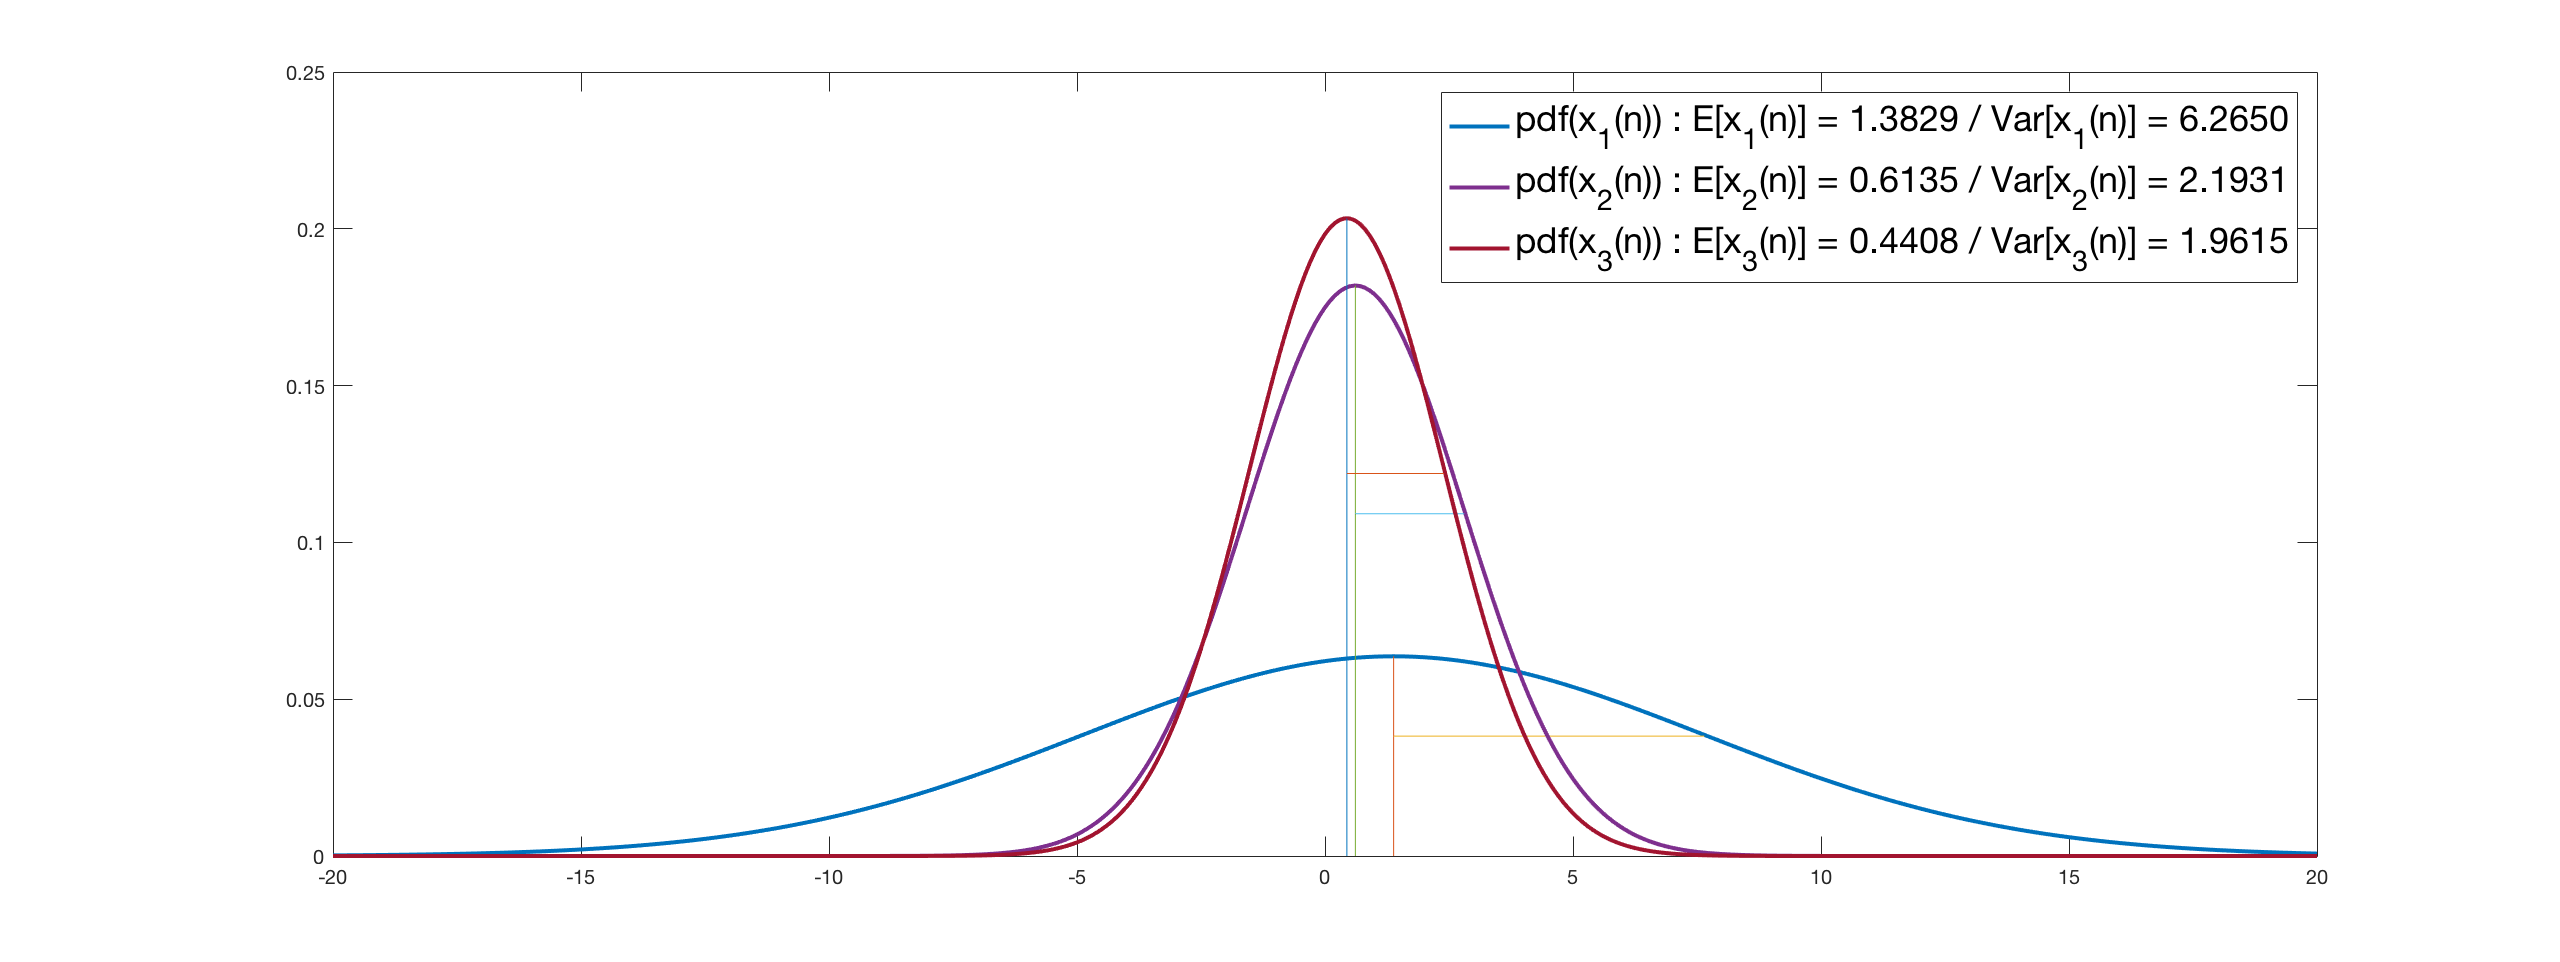
\includegraphics[scale = 0.1]{Task1}
	\caption{Visual representation of the three sequences $\{x_i(n)\}_{i=1}^3$ and estimation of their parameters}
\label{fig:Fig1}
\end{figure}
We can observe that the bigger $N_i$ is, better the approximation of the Gaussian parameters is. 

Thanks to the unbiased estimators, we know that we have, on average, the proper result but this is the fact the estimators \eqref{eq:Eq1} and \eqref{eq:Eq2} are consistant that explain this point $\begin{cases}Var[\hat{M}_{x}^2]= \frac{\sigma_x^2}{N_i} \\Var[\hat{S}_{x}^2]= 2\frac{\sigma_x^4}{N_i-1} \end{cases}$.
\end{multicols}


It is possible to approximate a Gaussian distribution as well as its parameters, with a degree of precision, with a long sequence.

\subsection*{Task 2}


Giving X and Y, two random variables with $X \hookrightarrow N(m_X, \sigma_X^2 = \sigma^2) $ and $Y \hookrightarrow N(m_Y, \sigma_Y^2= \sigma^2) $
\newline

The joint Gaussian distribution is :
\begin{equation} \label{eq:Eq5}
f_{XY}^{(i)}(x,y) = \frac { 1 }{ 2\pi \sigma^2 \sqrt { 1-{ \rho_i  }^{ 2 } }  } { e }^{ -\frac { { (x_i - m_X) }^{ 2 }-2\rho_i (x_i - m_X)(y_i-m_Y)+{ (y_i - m_Y) }^{ 2 } }{ 2 \sigma^2 (1-{ \rho_i  }^{ 2 }) }  }
\end{equation}
\newline

We want to study the impact of the correlation coefficient in the shape of the joint distribution. First we will visualize the shape of the joint distribution for two given correlation coefficient, then make a generalization.
\newline

\begin{multicols}{2}
For two sequences $\{x_i(n), y_i(n)\}_{i=1}^2$, the correlation coefficient $\rho_i$ between X and Y takes one of the values $\{0.25, 0.75\}$. We visualize the shape of the joint convolution for each sequence.
\begin{figure}[H]
	\centering
	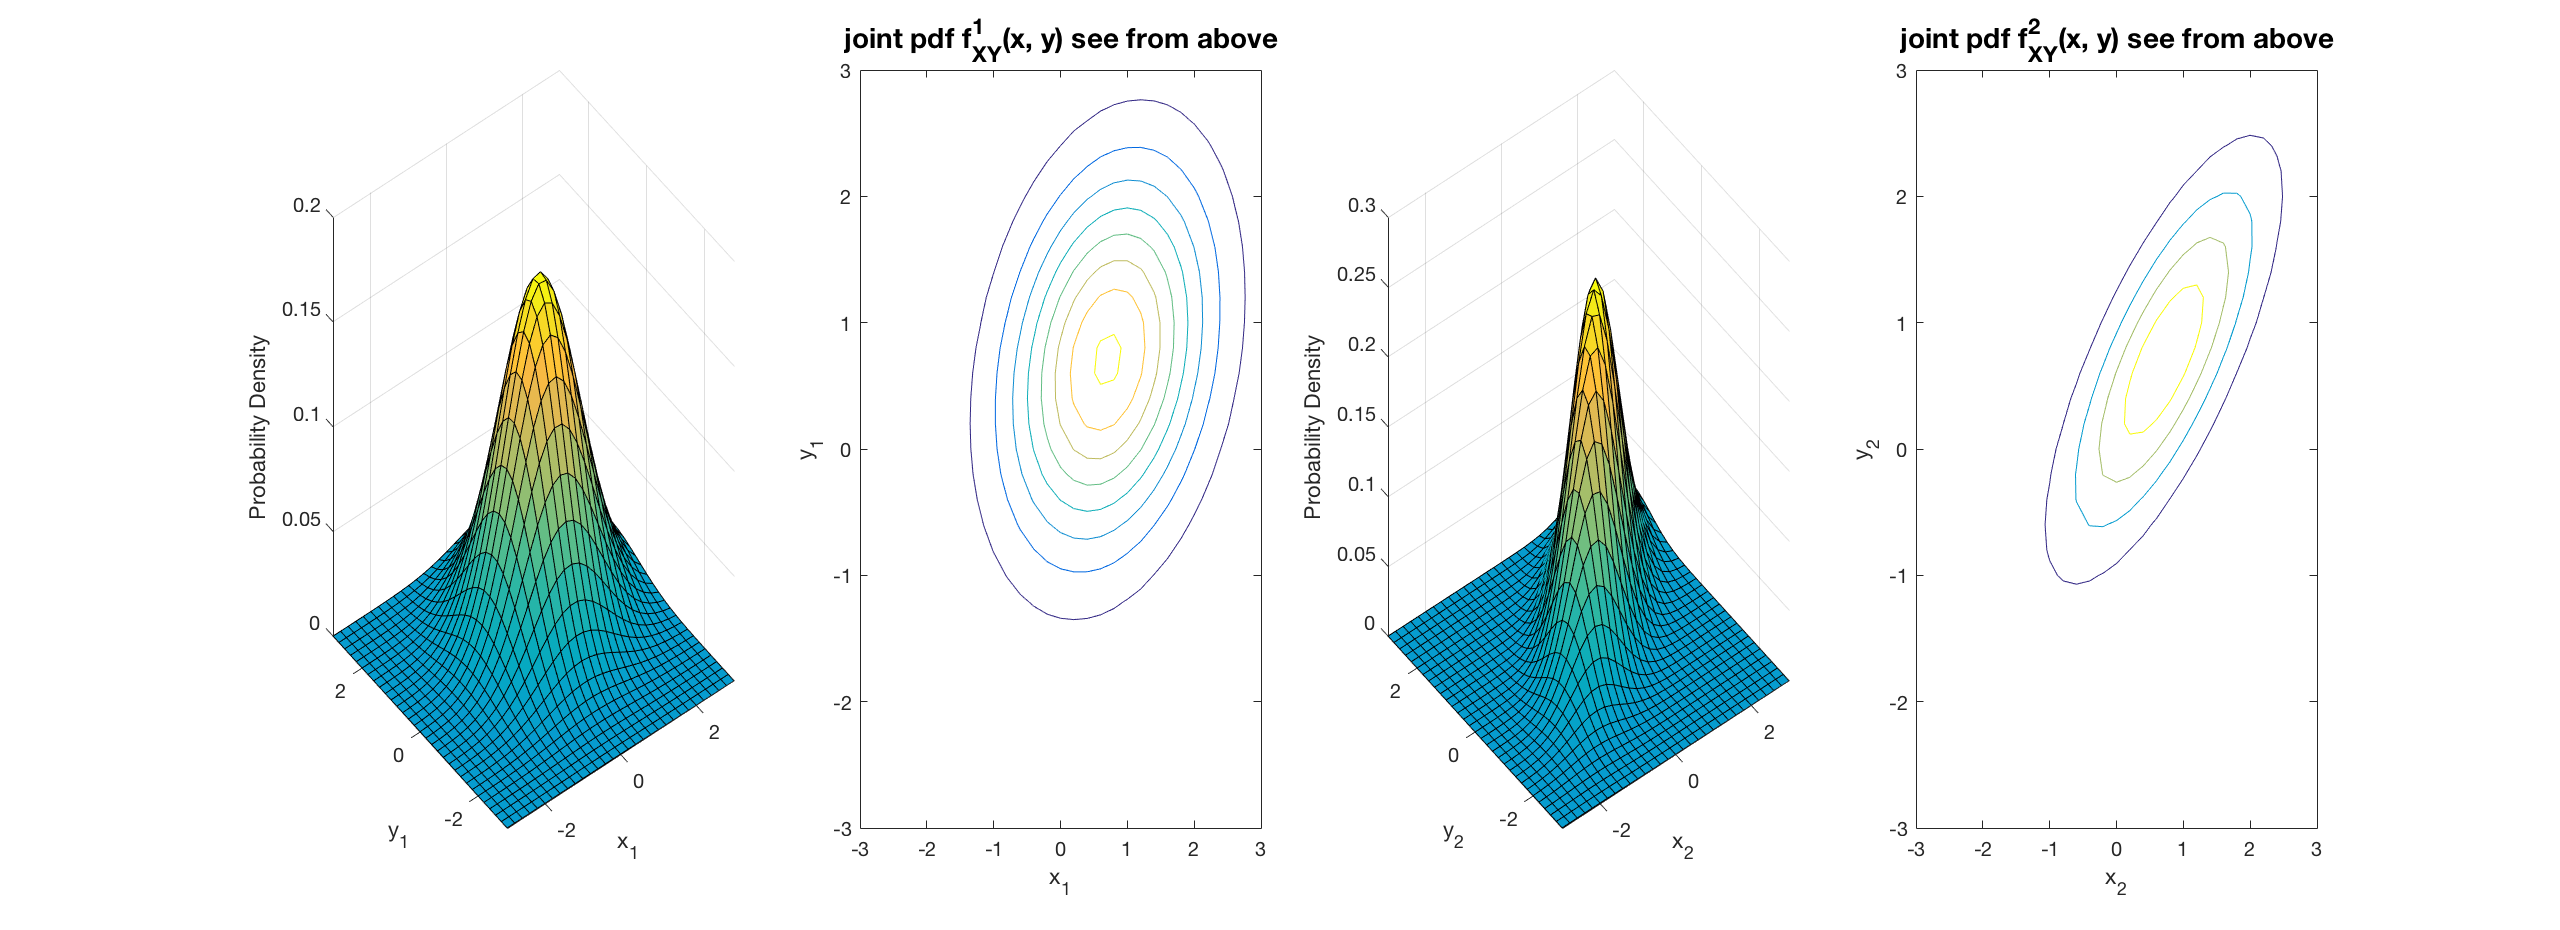
\includegraphics[scale = 0.1]{Task2.png}
	\caption{3D representation of the two pdfs and seen from above}
\label{fig:Fig2}
\end{figure}

\end{multicols}

To determine which correlation coefficient corresponds to which shape, we have to know that the correlation coefficient represents the relationship between the variable. In this case, the rounder the shape is, the weaker $|\rho_i|$ is; and the more linear the shape is and the stronger $|\rho_i|$ is.

So we can determine from Figure 2 that $\begin{cases}\rho = 0.25 \Rightarrow \{x_1(n), y_1(n)\} \\ \rho = 0.75 \Rightarrow \{x_2(n), y_2(n)\}
	\end{cases}$
\newline

Changing the sign of the correlation coefficient $\rho_i$ symmetrically inverts the shape of the distribution of the joint with respect to the mean of a variable.

\subsection*{Task 3}

Using \eqref{eq:Eq5}, we have $f_{XY}(x,y) = \frac { 1 }{ 2\pi \sigma^2 \sqrt { 1-{ \rho  }^{ 2 } }  } { e }^{ -\frac { { (x - m_X) }^{ 2 }-2\rho (x-m_X)(y-m_Y)+{ (y-m_Y) }^{ 2 } }{ 2 \sigma^2 (1-{ \rho  }^{ 2 }) }  }$
\newline
We want to determine some properties of the Gaussian distribution. We assume a correlation coefficient $\rho$, between $X$ and $Y$ , in all cases.
\begin{itemize}
	\item $f_{X|Y=y}(x) = \frac{f_{XY}(x,y)}{f_Y(y)} = \frac{1}{ \sigma \sqrt{1-\rho^2}\sqrt{2\pi}}e^{-\frac{[x - (m_X + \rho y - \rho m_Y))]^2}{2\sigma^2(1-\rho^2)}} $
	\newline
	\item Giving X and Y, two random variables with $X \hookrightarrow N(m_X, \sigma_X^2 = \sigma^2) $ and $Y \hookrightarrow N(m_Y, \sigma_Y^2= \sigma^2) $
		\newline
		
		The sum of two Gaussian is also Gaussian

		$E[X+Y] = E[X] + E[Y] = m_X + m_Y$

		$Var[X+Y] = Var[X] + Var[Y] + 2Cov(X,Y) = 2\sigma^2(1+\rho)$ 
		\newline
		
		We have $X+Y \hookrightarrow N(m_X + m_Y, 2\sigma^2(1+\rho)) $

		$f_{X+Y}(k) = \frac{1}{\sqrt{4\pi\sigma^2(1+\rho)}}e^{-\frac{(k-m_X-m_Y)^2}{4\sigma^2(1+\rho)}}$

	\item Giving X and Y, two random variables with $X \hookrightarrow N(m_X, \sigma_X^2 = \sigma^2) $ and $Y \hookrightarrow N(m_Y, \sigma_Y^2= \sigma^2) $
		\newline
		
		The sum of two Gaussian is also Gaussian

		$E[X-Y] = E[X] - E[Y] = m_X - m_Y$

		$Var[X-Y] = Var[X] + Var[Y] - 2Cov(X,Y) = 2\sigma^2(1-\rho)$ 
		\newline
		
		We have $X-Y \hookrightarrow N(m_X - m_Y, 2\sigma^2(1-\rho)) $
		
		$f_{X-Y}(k) = \frac{1}{\sqrt{4\pi\sigma^2(1-\rho)}}e^{-\frac{(k-m_X+m_Y)^2}{4\sigma^2(1-\rho)}}$ 

\end{itemize}

\subsection*{Conclusion}
We have seen in this section that to estimate the parameter of a Gaussian distribution, the longer the sequence is, the better the estimation is. 
We have also studied some properties of the joint Gaussian distribution, in particular, the impact of the correlation coefficient which shape of the joint distribution.



\section{System Models with Gaussian Noise}

This section presents different models of Gaussian noise systems. We will interpret the impact of noise on the estimation of the parameters of the desired signal.

\subsection*{Task 4}

In this task, we want to transfer two sinusoïdal signals but the transmission is disturbed by a Gaussian noise. 

We have two possible outcomes, H0: $y_0(n) = w(n)$ and H1: $y_1(n) = \sum_{k=0}^{1}{sin(2\pi \nu_k n + \phi_k)} + w(n)$. To determine which output sequence contains the sinusoïdal information, we estimate the power spectrum through a technic called periodogram and we get the results below :

\begin{multicols}{2}
\begin{figure}[H]
	\centering
	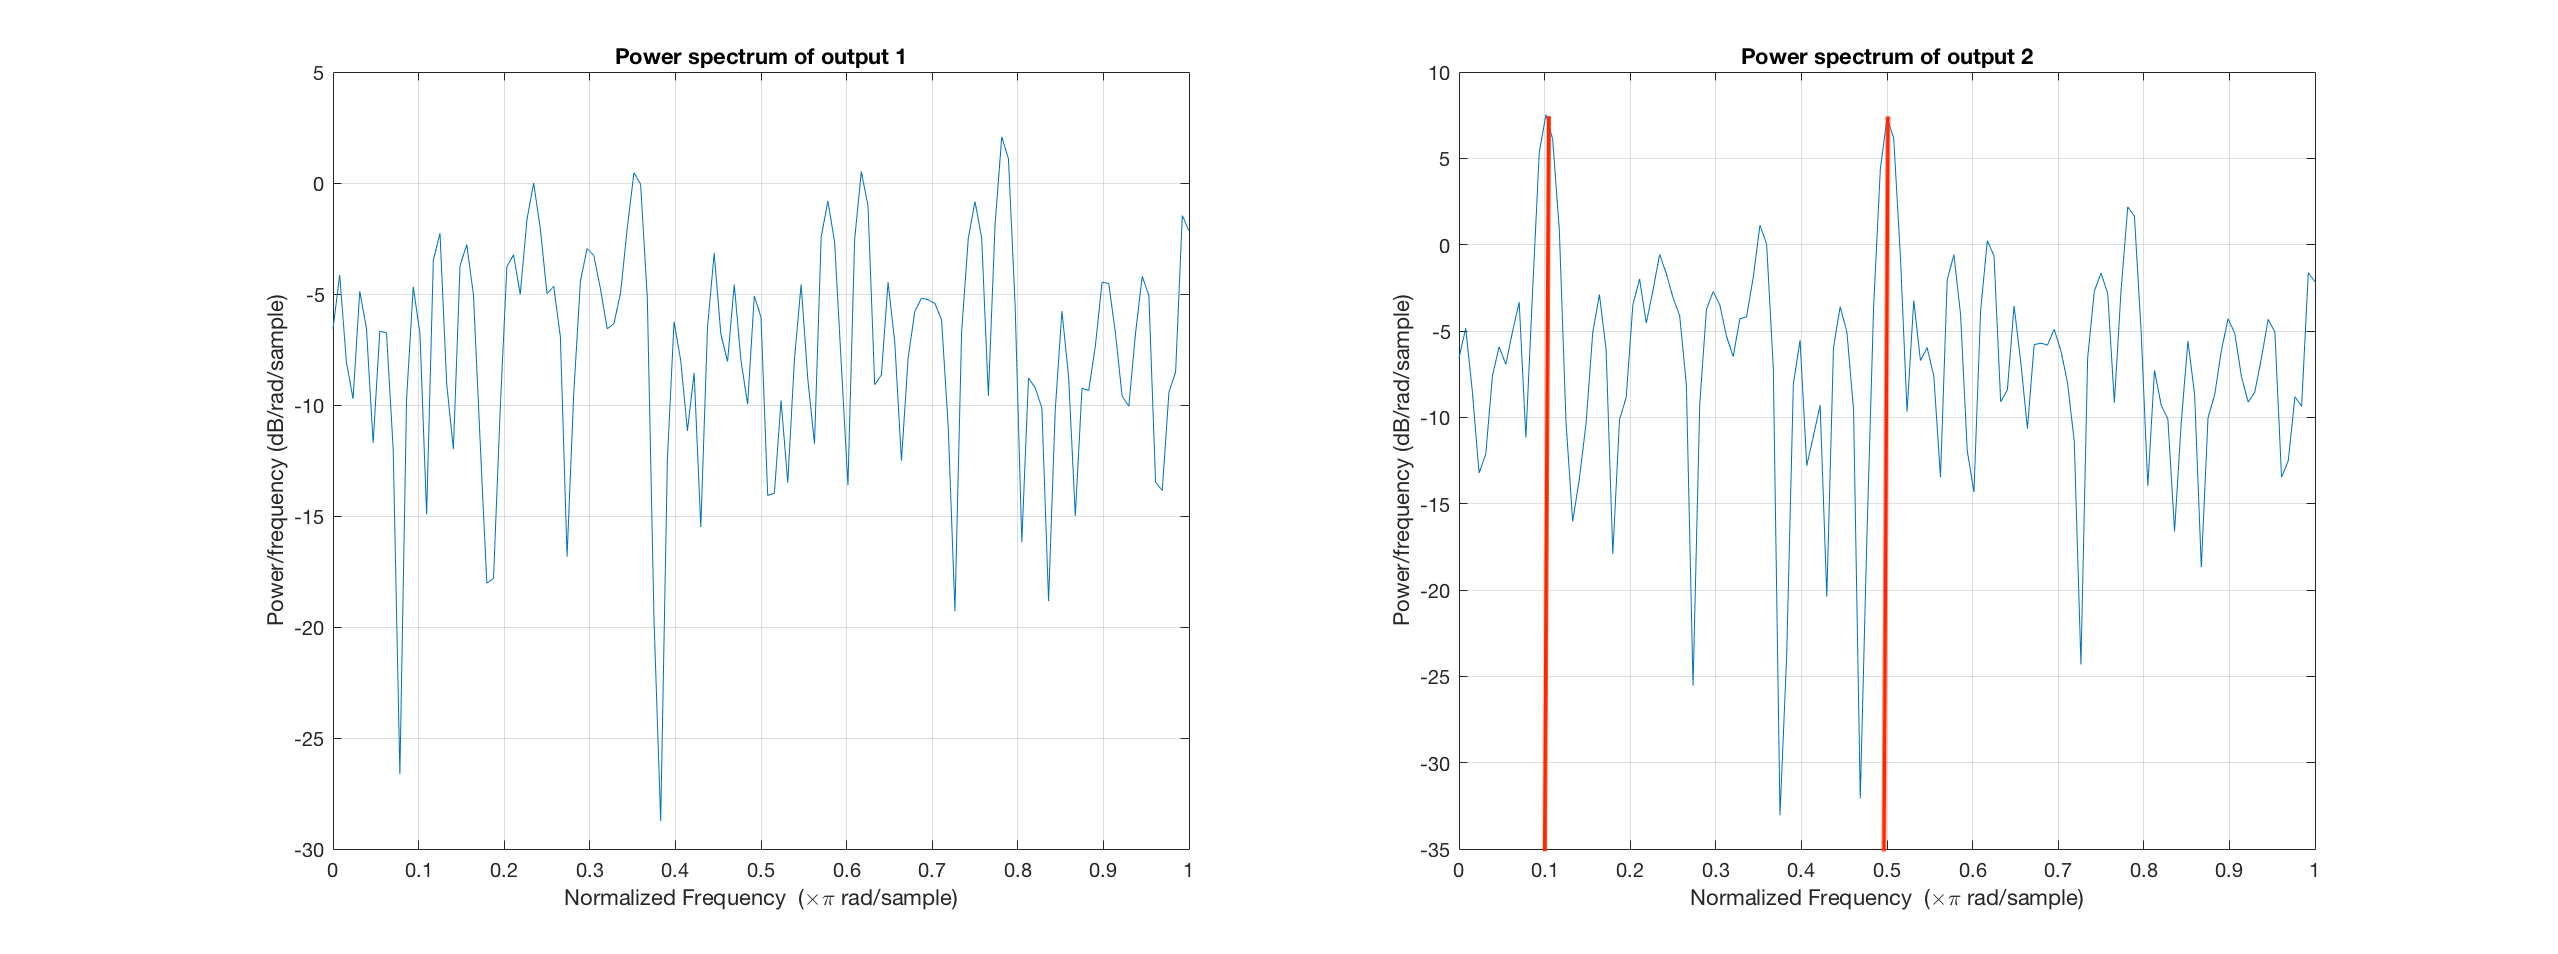
\includegraphics[scale = 0.11]{Task4.png}
	\caption{Periodogram of the different outputs}
\label{fig:Fig4}
\end{figure}

The two sinusoidal signals have normalized (with the sampling frequency fs) frequencies $\nu_0 = 0.05$ and $\nu_1 = 0.25$ and initial phases $\varphi_0$ and $\varphi_1$, respectively. So the power spectrum of the output with the sinusoïdal information must contains power peaks on the normalized frequencies $\nu_0$ and $\nu_1$.
\end{multicols}




On the power spectrum of output 2, we can see that there is two power peaks on the normalized frequencies $2*\nu_0 = 0,1$ and $2*\nu_1 = 0,5$. (We have $2*\nu_0 = 0,1$ and $2*\nu_1 = 0,5$ because on the periodogram the frequencies are normalized by $\pi$ rad/sample instead of $2\pi$ rad/sample).
\newline

So we have, the power spectrum of output 1 is the power spectrum of H0 and the power spectrum of output 2 is the power spectrum of H1.
\newline

For a white noise, the estimation accuracy of the frequencies depends on the signal noise ratio (SNR). If the power of the noise is stronger than the power of the signal, it will be difficult to estimate the frequencies. It is therefore necessary to keep a large SNR to find the required information in a periodogram.




\subsection*{Task 5}

Sometimes, the transmission could be disturbed by a colored noise. We want to analyze the power spectrum to see the impact of the noise on the estimated power spectrum.

\begin{multicols}{2}
\begin{figure}[H]
	\centering
	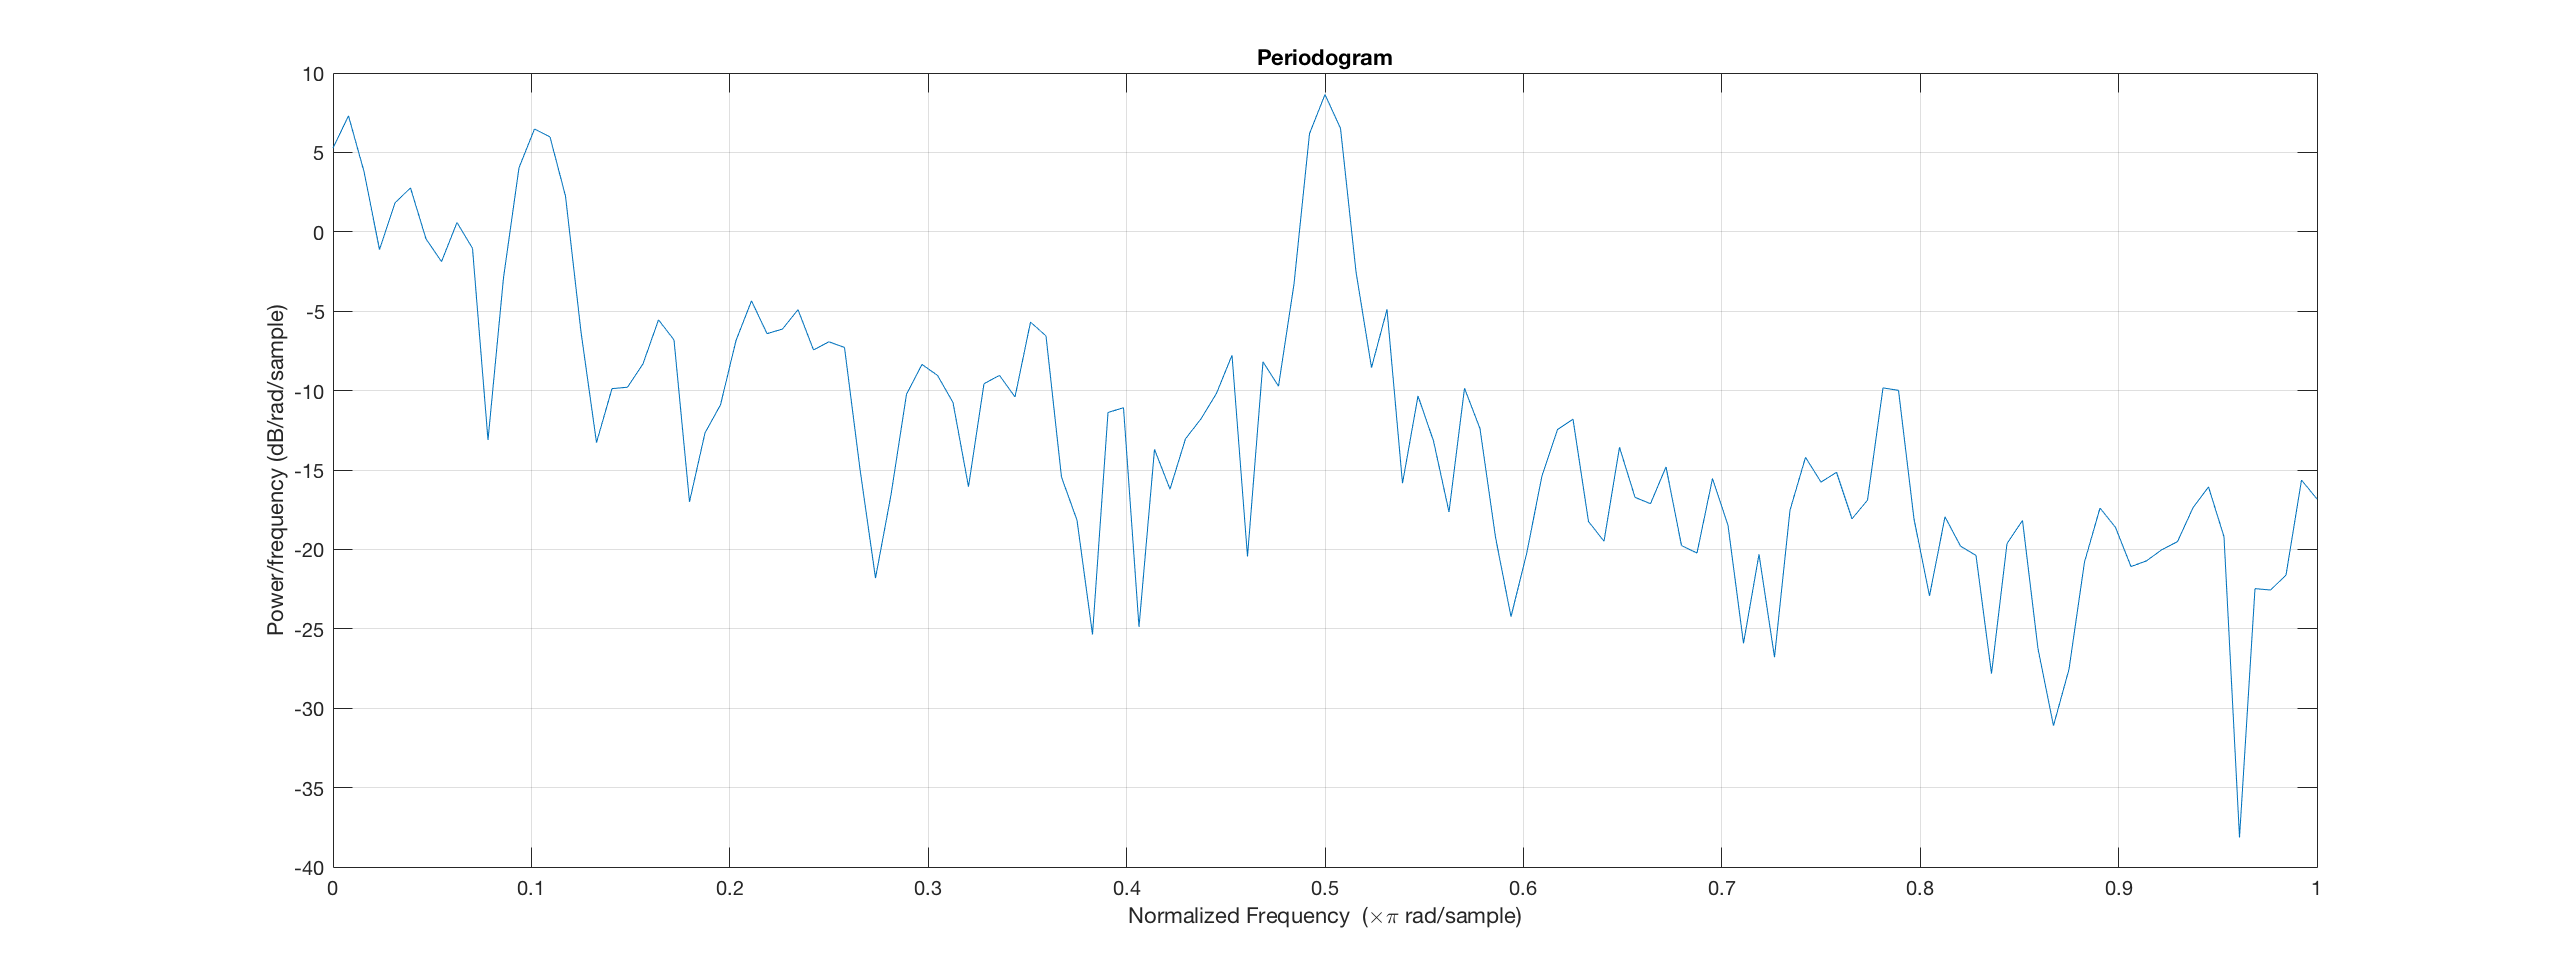
\includegraphics[scale = 0.1]{Task5.png}
	\caption{Periodogram}
\label{fig:Fig5}
\end{figure}
Most of the noise is situated in the low frequencies area so it is difficult to distinguish the low frequency $2*\nu_0 = 0,1$ of the sinusoïdal signal. On the other hand we can properly distinguish the frequency at $2*\nu_1 = 0,5$ because the noise power is weak in this frequency range.
\end{multicols}


For colored noise, the estimation accuracy of the frequencies is difficult if the frequencies are situated in the low frequencies area.

\subsection*{Task 6}
$x_1(n) = \alpha x_1(n-1) + z(n)$

$x_2(n) = \sum_{k = 0}^{+\infty}{h_2(n)x_1(n-k)}$

We want to determine the power spectra of the signals $x_1(n)$ and $x_2(n)$.

\begin{equation} \label{eq:Eq6}
	R_{x}(\nu) = F[r_{x}(k)]
\end{equation}

For a linear time invariant system we have :
\begin{equation} \label{eq:Eq7}
	R_{output}(\nu) = |H(\nu)|^2R_{input}(\nu)
\end{equation}

To determine the power spectrum we will use the formula \eqref{eq:Eq6} and \eqref{eq:Eq7}.

\begin{itemize}
	\item $x_1(n) = \alpha x_1(n-1) + z(n)$

$\begin{cases} \sigma_{x_1}^2 = \frac{\sigma_z^2}{1 - \alpha^2} \\ r_{x_1}(k) = \alpha^{|k|}r_{x_1}(0) = \alpha^{|k|}\sigma_{x_1}^2 \end{cases} \Leftrightarrow  r_{x_1}(k) = \alpha^{|k|}\frac{\sigma_z^2}{1 - \alpha^2}$
\newline

We deduce that $R_{x_1}(\nu) = F[r_{x_1}(k)] = \frac{\sigma_z^2}{1 + \alpha^2 - 2\alpha cos(2\pi\nu)} = \frac{1}{\frac{17}{16} - \frac{1}{2}cos(2\pi\nu)}$

	\item $x_2(n) = \sum_{k = 0}^{+\infty}{h_2(n)x_1(n-k)} = (h_2 * x_1)(n)$
\newline

We have a linear time invariant system so we can use the formula \eqref{eq:Eq7} and the formula (7.19) in [1] :

$H(\nu) = F[h_2(n)] = \frac{1}{1 - \beta e^{-j2\pi\nu}}$
\newline

We deduce that $R_{x_2}(\nu) = |H(\nu)|^2R_{x_1}(\nu) = \frac{\sigma_z^2}{(1-2\beta cos(2\pi\nu) + \beta^2)(1 - 2\alpha cos(2\pi\nu) + \alpha^2)} = \frac{1}{(\frac{17}{16} - \frac{1}{2}cos(2\pi\nu))^2}$

\end{itemize}

\begin{figure}[H]
	\centering
	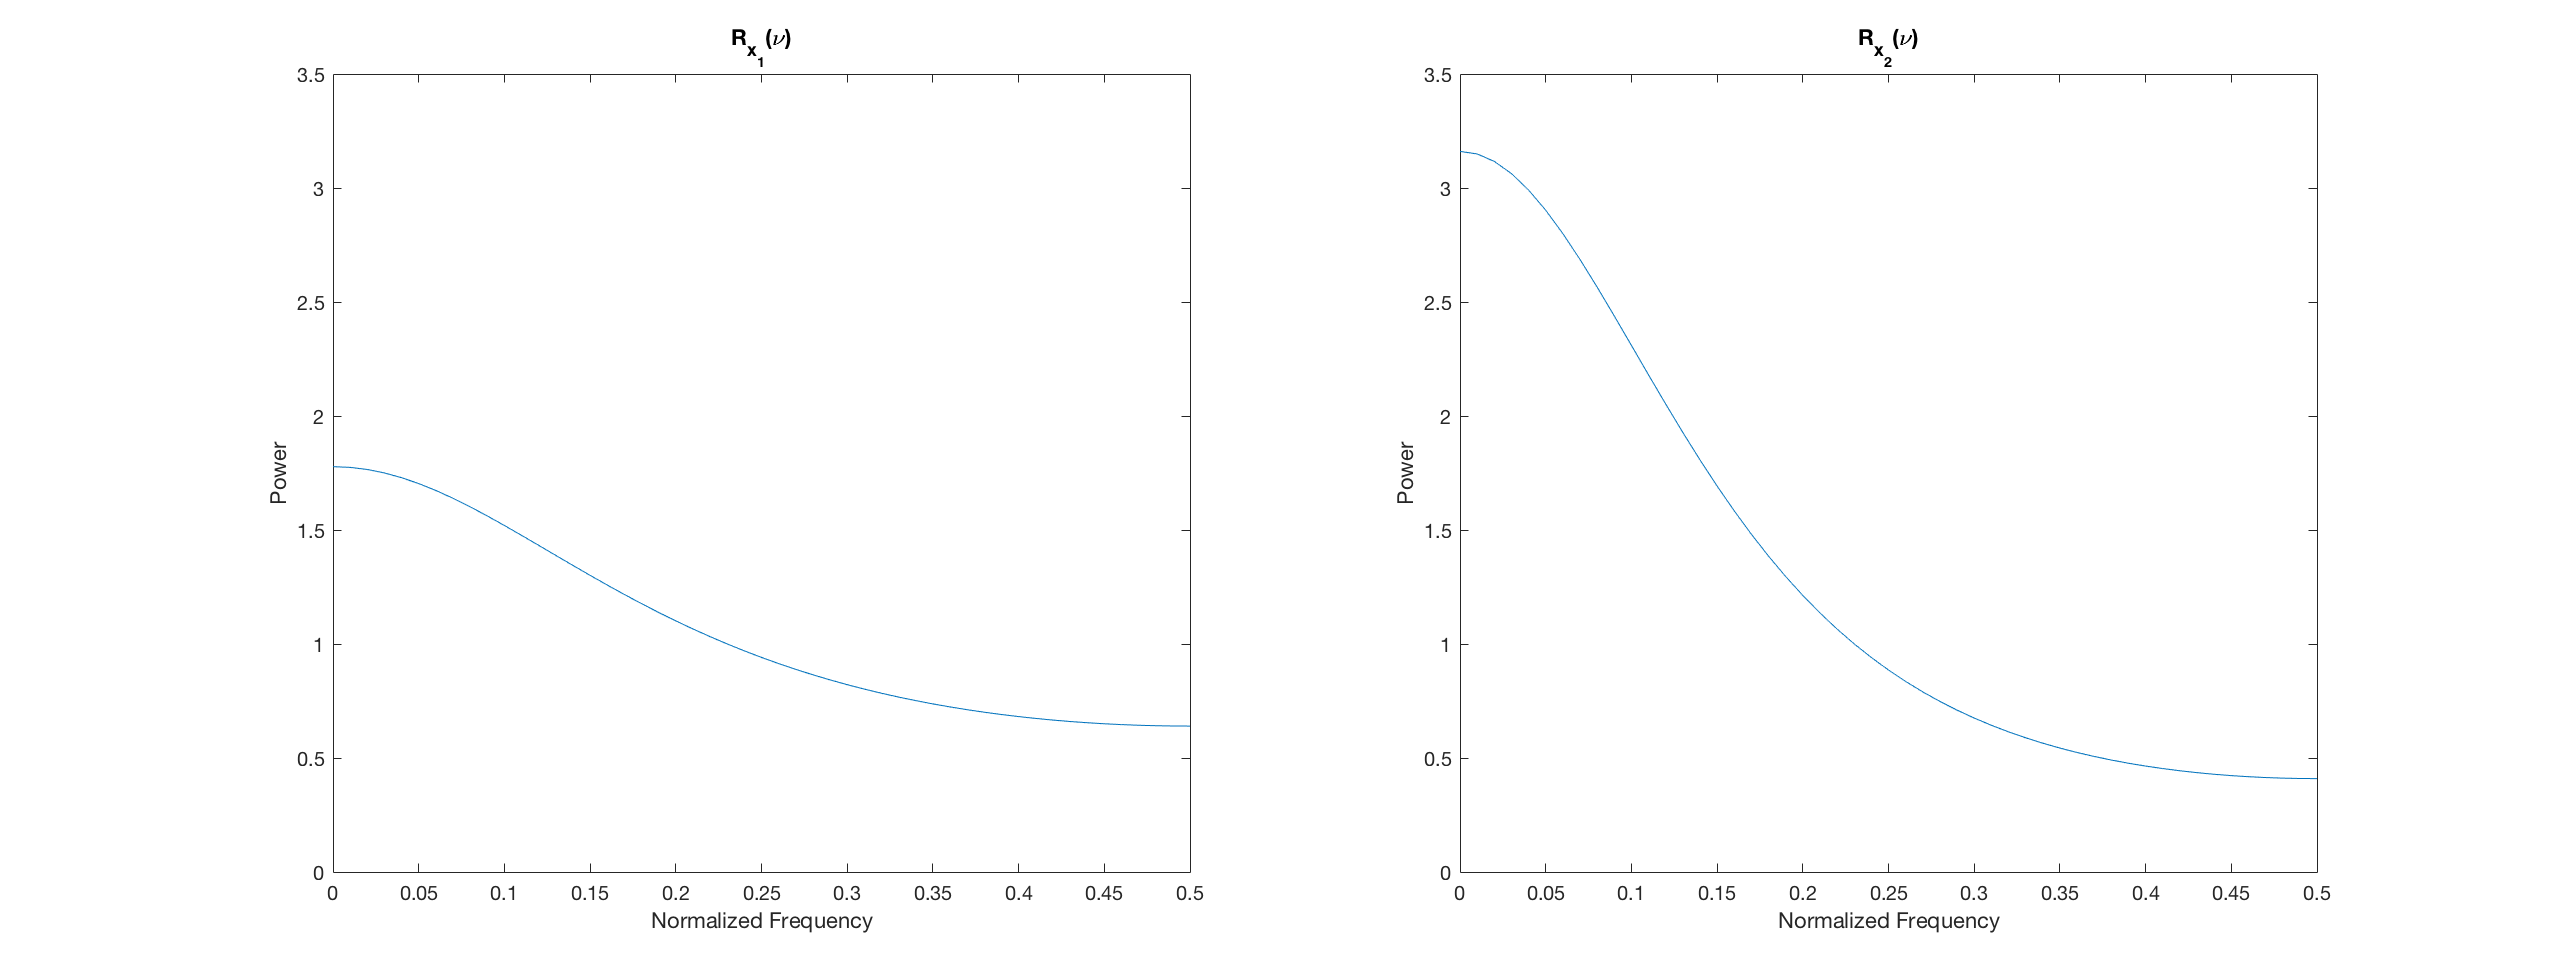
\includegraphics[scale = 0.1]{Task6.png}
	\caption{Power spectra of $x_1(n)$ and $x_2(n)$}
\label{fig:Fig6}
\end{figure}



\subsection*{Task 7}

In the last task, we derive $R_{x_2}(\nu)$ without knowing $r_{x_2}(k)$. Now we want to determine $r_{x_2}(k)$. For that we will use the inverse Fourier transform of the power spectrum.

\begin{equation} \label{eq:Eq8}
	r_{x_2}(k) = F^{-1}[R_{x_2}(\nu)]
\end{equation}

\begin{multicols}{2}
We obtain $r_{x_2}(k) = \sigma_z^2 \frac{1}{(1-\beta^2)(1-\alpha^2)} \beta^{|k|}*\alpha^{|k|}$

$r_{x_2}(k) = \frac{256}{225}(0.25)^{|k|}*0.25^{|k|}$

$r_{x_2}(k) = \frac{256}{225} \frac{0.25^{|k|}(|k| + 1) + 0.25^{|k| + 2}(|k|-1)}{1 - 0.25^2}$

$r_{x_2}(k) \approx 0.25^{|k|} (|k|+1)$
\begin{figure}[H]
	\centering
	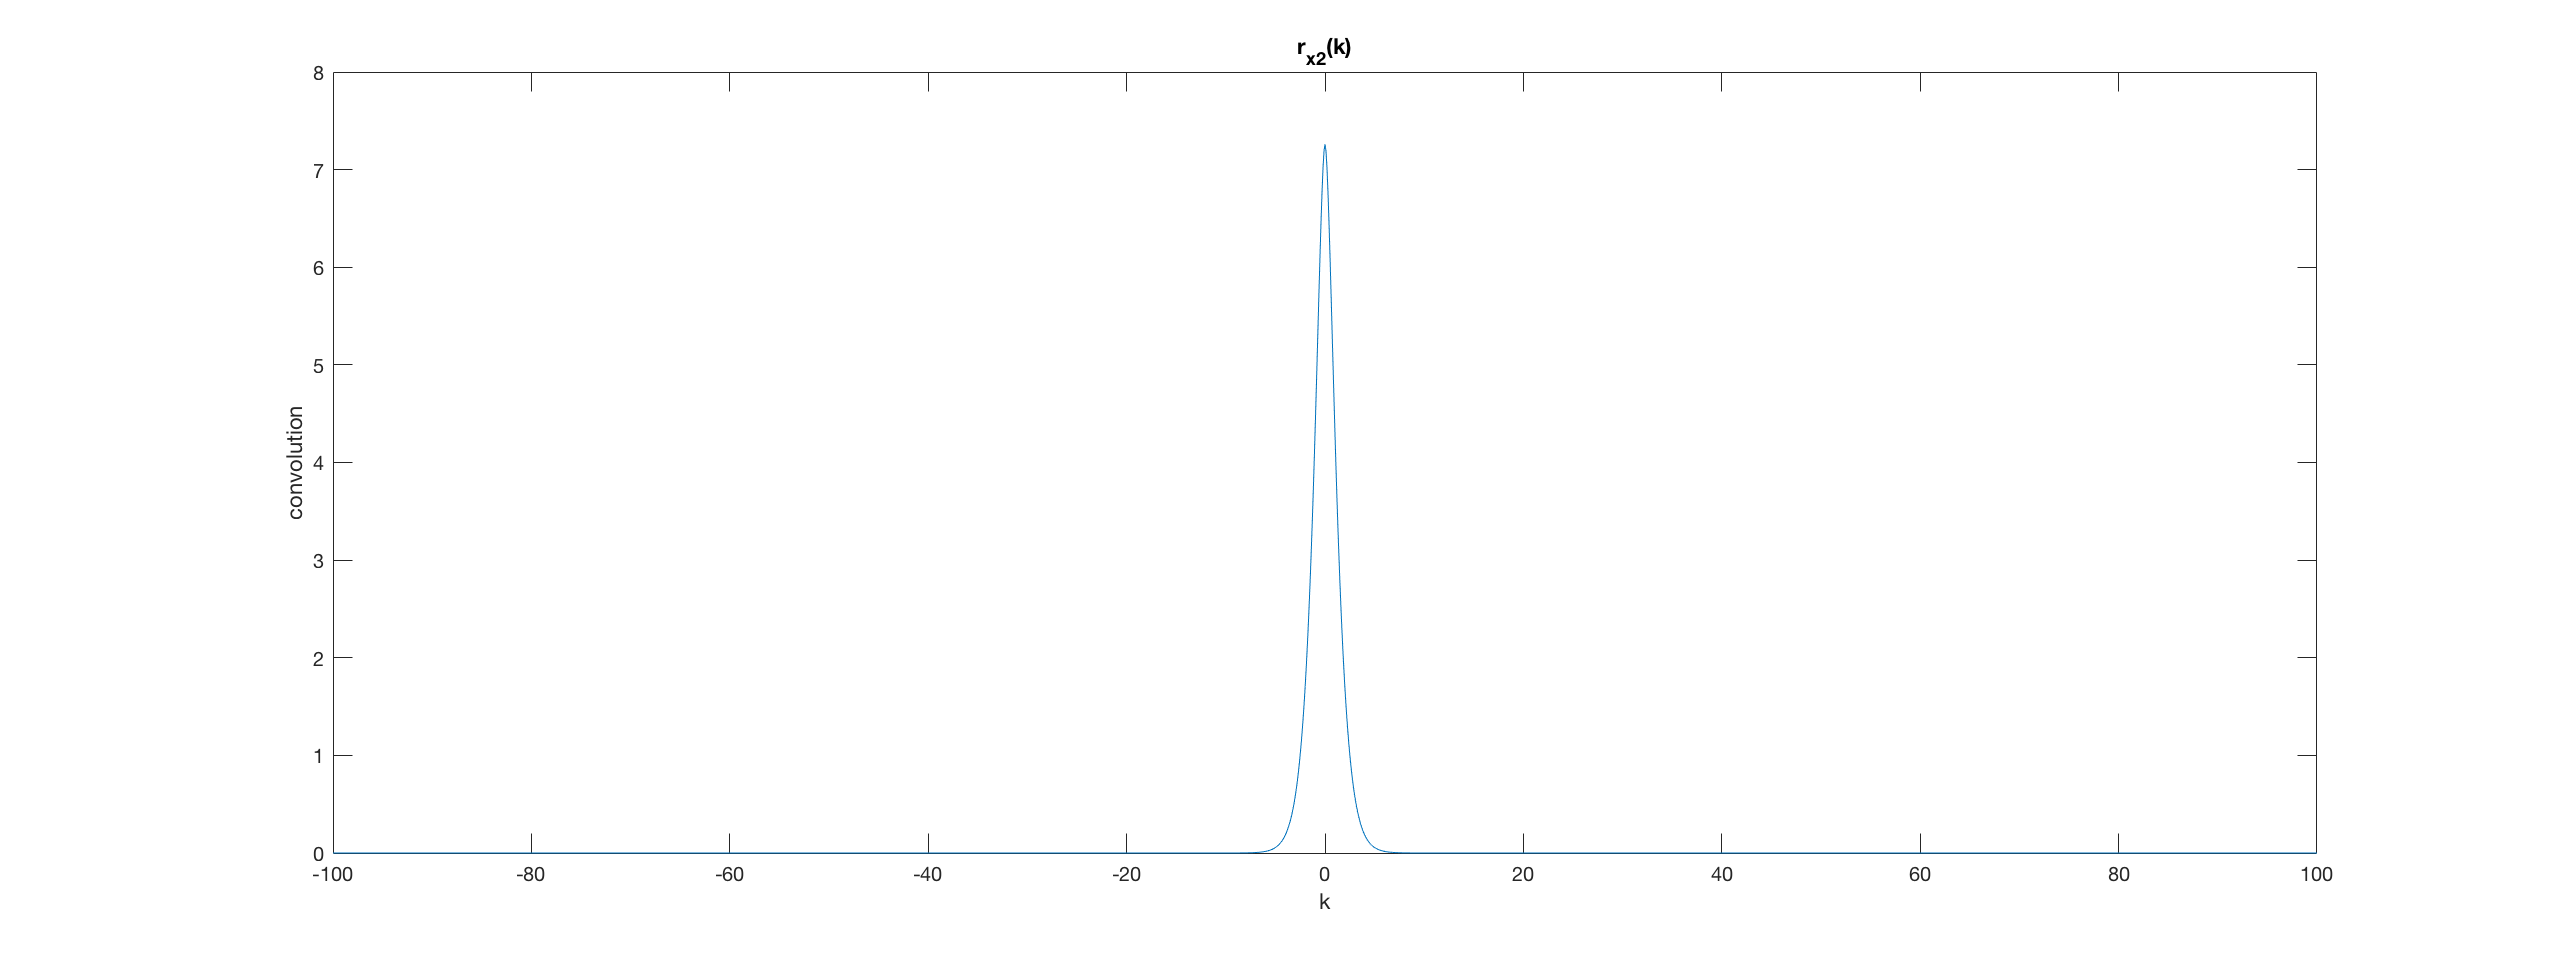
\includegraphics[scale = 0.11]{Task7.png}
	\caption{ACF of $x_2(n)$}
\label{fig:Fig7}
\end{figure}
\end{multicols}

\subsection*{Conclusion}

This section has allowed us to understand how to estimate the required information in a system model with a Gaussian noise. In a power study, it is important to have a large SNR in order to recover the information in the power spectrum.

\section{Conclusions}
In this project, we have seen some properties of a Gaussian distribution and the impact of its parameters. We have also seen how to estimate the required information in the presence of a Gaussian noise (white or colored noise).

The SNR, sequence length and correlation coefficient are important information to know because a poor knowledge of this information can lead to a bad study with misinterpretations.
\newline

These concepts are important because of system modeling in electronics and signal processing which often uses a Gaussian noise to model the noise present.

\section{References}
[1]\quad Collection of Formula in Signal Processing, KTH, 2016


%\newpage
%\section{Appendix}
%
%\subsection*{Task 1}
%
%\begin{itemize}
%	\item Mean estimator
%
%$\hat{M}_x = \frac{1}{N_i}\sum_{n = 1}^{N_i}{X_i(n)}$
%\newline
%\newline
%$E[\hat{M}_x] = E[\frac{1}{N_i}\sum_{n = 1}^{N_i}{X_i(n)}]$
%
%$E[.]$ is a linear operator $\Rightarrow E[\hat{M}_x] = \frac{1}{N_i}\sum_{n = 1}^{N_i}{E[X_i(n)]} = m_X$
%\newline
%
%
%$Var[\hat{M}_x] = Var[\frac{1}{N_i}\sum_{n = 1}^{N_i}{X_i(n)}]$
%
%$X_i(n)$ is an i.i.d sequence $\Rightarrow Var[\hat{M}_x] = \frac{1}{N_i^2}\sum_{n = 1}^{N_i}{Var[X_i(n)]} = \frac{\sigma_X}{N_i} $
%
%	\item Variance estimator
%	
%$\hat{S}_{x}^2 = k\sum_{n = 1}^{N_i}{(X_i(n) - \hat{M}_x)^2}$
%\newline
%\newline
%
%$X_i(n)$ is an i.i.d sequence, if $X_i \hookrightarrow N(m_X, \sigma_X^2)$ so $\sum_{n = 1}^{N_i}{(\frac{X_i(n) - m_X}{\sigma_X})^2 \hookrightarrow \chi_{N_i - 1}^2}$
%
%So we have $\begin{cases} E[\sum_{n = 1}^{N_i}{(\frac{X_i(n) - m_X}{\sigma_X}})^2] = N_i - 1 \\ Var[\sum_{n = 1}^{N_i}{(\frac{X_i(n) - m_X}{\sigma_X})^2}] = 2(N_i - 1)\end{cases}$ 
%\newline
%
%$\hat{S}_{x}^2 = k\sum_{n = 1}^{N_i}{(X_i(n) - \hat{M}_x)^2} \Leftrightarrow \frac{\hat{S}_{x}^2}{k\sigma_X^2} = \sum_{n = 1}^{N_i}{(\frac{X_i(n) - \hat{M}_x}{\sigma_X})^2}$
%
%$\Rightarrow \begin{cases} E[\frac{\hat{S}_{x}^2}{k\sigma_X^2}] = N_i - 1 \\ Var[\frac{\hat{S}_{x}^2}{k\sigma_X^2}] = 2(N_i - 1)\end{cases}$
%$\Leftrightarrow \begin{cases} E[\hat{S}_{x}^2] = k\sigma_X^2(N_i - 1) \\ Var[\hat{S}_{x}^2] = 2k^2\sigma_X^4(N_i - 1) \end{cases}$
%\newline
%
%To have an unbiased estimator $k$ must be equal to $\frac{1}{N_i - 1}$
%
%$\Rightarrow \begin{cases} E[\hat{S}_{x}^2] = \sigma_X^2 \\ Var[\hat{S}_{x}^2] = 2\frac{\sigma_X^4}{N_i - 1} \end{cases}$
%
%\end{itemize}
%
%\subsection*{Task 6}
%
%
%$x_1(n) = \alpha x_1(n-1) + z(n)$
%\newline
%
%For $|k| > 1$, $r_{x_1}(k) = E[x_1(n)x_1(n-k)]$
%
%$\Leftrightarrow r_{x_1}(k) = E[(\alpha x_1(n-1) + z(n))x_1(n-k)]$
%
%E[.] is a linear operator so $r_{x_1}(k) = \alpha E[x_1(n-1)x_1(n-k)] + E[z(n)x_1(n-k)]$
%
%z(n) is a white noise so $E[z(n)x_1(n-k)] = 0$
%
%$r_{x_1}(k) = \alpha E[x_1(n-1)x_1(n-k)] = \alpha E[x_1(n-1)x_1(n - 1- (k-1))]$
%
%$\Leftrightarrow r_{x_1}(k) = \alpha r_{x_1}(k-1)$
%
%By recurrence $r_{x_1}(k) = \alpha^{|k|}r_{x_1}(0) = \alpha^{|k|}Var[x_1(n)]$
%
%For k = 0, this formula is still true so for any $k \in N$,  $r_{x_1}(k) = \alpha^{|k|}Var[x_1(n)]$
%\newline
%
%$Var[x_1(n)] = Var[\alpha x_1(n-1) + z(n)]$
%
%$\Leftrightarrow Var[x_1(n)] = \alpha^2 Var[x_1(n-1)] + Var[z(n)]$
%
%$Var[x_1(n)] = Var[x_1(n-1)]$ and $Var[z(n)] = \sigma_z^2$ so $Var[x_1(n)] = \frac{\sigma_z^2}{1-\alpha^2}$
%\newline
%
%We get $r_{x_1}(k) = \alpha^{|k|}\frac{\sigma_z^2}{1-\alpha^2}$
%\newline
%
%We use \eqref{eq:Eq6} to get the power spectrum :
%
%$R_{x_1}(\nu) = \sum_{k = -\infty}^{\infty}{r_{x_1}(k) e^{-j2\pi \nu k}} = \sum_{k = -\infty}^{\infty}{\alpha^{|k|}\frac{\sigma_z^2}{1-\alpha^2} e^{-j2\pi \nu k}}$
%
%$\Leftrightarrow R_{x_1}(\nu) = \frac{\sigma_z^2}{1 - \alpha^2}[\sum_{-\infty}^{0}{\alpha^{|k|}e^{-j2\pi \nu k}} + \sum_{0}^{\infty}{\alpha^{|k|}e^{-j2\pi \nu k}} - 1]$
%
%$\Leftrightarrow R_{x_1}(\nu) = \frac{\sigma_z^2}{1 - \alpha^2}[\sum_{0}^{\infty}{(\alpha e^{j2\pi \nu})^k} + \sum_{0}^{\infty}{(\alpha e^{-j2\pi \nu})^k} - 1]$
%
%As $|\alpha| < 1$, we can affirm the existence of $\sum_{0}^{\infty}{(\alpha e^{j2\pi \nu})^k}$ and $\sum_{0}^{\infty}{(\alpha e^{-j2\pi \nu})^k}$
%
%$\Rightarrow \begin{cases}
%	\sum_{0}^{\infty}{(\alpha e^{j2\pi \nu})^k} = \frac{1}{1 - \alpha e^{j2\pi \nu}}\\
%	\sum_{0}^{\infty}{(\alpha e^{-j2\pi \nu})^k} = \frac{1}{1 - \alpha e^{-j2\pi \nu}}
%\end{cases}$
%
%So $R_{x_1}(\nu) = \frac{\sigma_z^2}{1 - \alpha^2}[\frac{1}{1 - \alpha e^{j2\pi \nu}} + \frac{1}{1 - \alpha e^{-j2\pi \nu}} - 1]$
%
%$\Leftrightarrow R_{x_1}(\nu) = \frac{\sigma_z^2}{1 + \alpha^2 - 2\alpha cos(2\pi\nu)} = \frac{1}{\frac{17}{16} - \frac{1}{2}cos(2\pi\nu)}$
%
%\subsection*{Task 7}
%$R_{x_2}(\nu) = \frac{\sigma_z^2}{(1-2\beta cos(2\pi\nu) + \beta^2)(1 - 2\alpha cos(2\pi\nu) + \alpha^2)}$
%	\newline
%	
%We use the formula (7.21) in [1]
%\newline
%
%$\Rightarrow F^{-1}[\frac{1 - a^2}{1 - 2a cos(2\pi\nu) + a^2}] = a^{|k|}$
%\newline
%
%So $r_{x_2}(k) = F^{-1}[R_{x_2}(\nu)] = \sigma_z^2 F^{-1}[\frac{1}{(1-2\beta cos(2\pi\nu) + \beta^2)(1 - 2\alpha cos(2\pi\nu) + \alpha^2)}]$
%
%$\Leftrightarrow r_{x_2}(k) = \sigma_z^2 F^{-1}[\frac{1}{1-2\beta cos(2\pi\nu) + \beta^2}]*F^{-1}[\frac{1}{1 - 2\alpha cos(2\pi\nu) + \alpha^2}]$
%
%$\Leftrightarrow r_{x_2}(k) = \sigma_z^2 \frac{1}{1 - \beta^2}F^{-1}[\frac{1 - \beta^2}{1-2\beta cos(2\pi\nu) + \beta^2}]*\frac{1}{1-\alpha^2}F^{-1}[\frac{1 - \alpha^2}{1 - 2\alpha cos(2\pi\nu) + \alpha^2}]$
%\newline
%
%$\Leftrightarrow r_{x_2}(k) = \sigma_z^2 \frac{1}{(1-\beta^2)(1-\alpha^2)} \beta^{|k|}*\alpha^{|k|} = \frac{256}{225}(0.25)^{|k|}*0.25^{|k|}$





\end{document}
